
\renewcommand{\FileName}{titanic}

\begin{frame}
\frametitle{Survival on the \textit{Titanic}}
%\begin{itemize}
%\item Survival on the \textit{Titanic}
%\item Lifeboats on the \textit{Titanic}
%\end{itemize}

Survival on the \textit{Titanic}:  2201 passengers, classified by 
Class, Gender, Age, survived.  Data from:
\begin{itemize*}
\item \citet{Mersey:1912}, \textit{Report on the loss of the ``Titanic'' S.S.}
\item \citet{Dawson:95}
\end{itemize*}
\vspace{-10pt}
%%
%% Table titanic written by md2tex 09APR99 14:57
%%
\begin{table}[htb]
 \caption{Survival on the Titanic}
 \label{tab:titanic}
 \begin{center}
  \begin{tabular}{|lll|rrrr|}
   \hline
 &  &  & \multicolumn{4}{c|}{\bfseries\large Class   }\rule{0in}{2.5ex}\\
{\bfseries\large Gender     } & {\bfseries\large Age     } & {\bfseries\large Survived} & 1st      & 2nd      & 3rd      & Crew     \\
   \hline
Male     & Adult   & Died       &    118 &    154 &    387 &    670 \\
Female   &         &            &      4 &     13 &     89 &      3 \\
[4pt]
Male     & Child   &            &      0 &      0 &     35 &      0 \\
Female   &         &            &      0 &      0 &     17 &      0 \\
[4pt]
Male     & Adult   & Survived   &     57 &     14 &     75 &    192 \\
Female   &         &            &    140 &     80 &     76 &     20 \\
[4pt]
Male     & Child   &            &      5 &     11 &     13 &      0 \\
Female   &         &            &      1 &     13 &     14 &      0 \\
   \hline
  \end{tabular}
 \end{center}
\end{table}


Order of variables in mosaics:  Class, Gender, Age, Survival

\end{frame}


\begin{frame}
\frametitle{Survival on the \textit{Titanic}: Background variables}

 \begin{minipage}[c]{.55\dispwidth}
  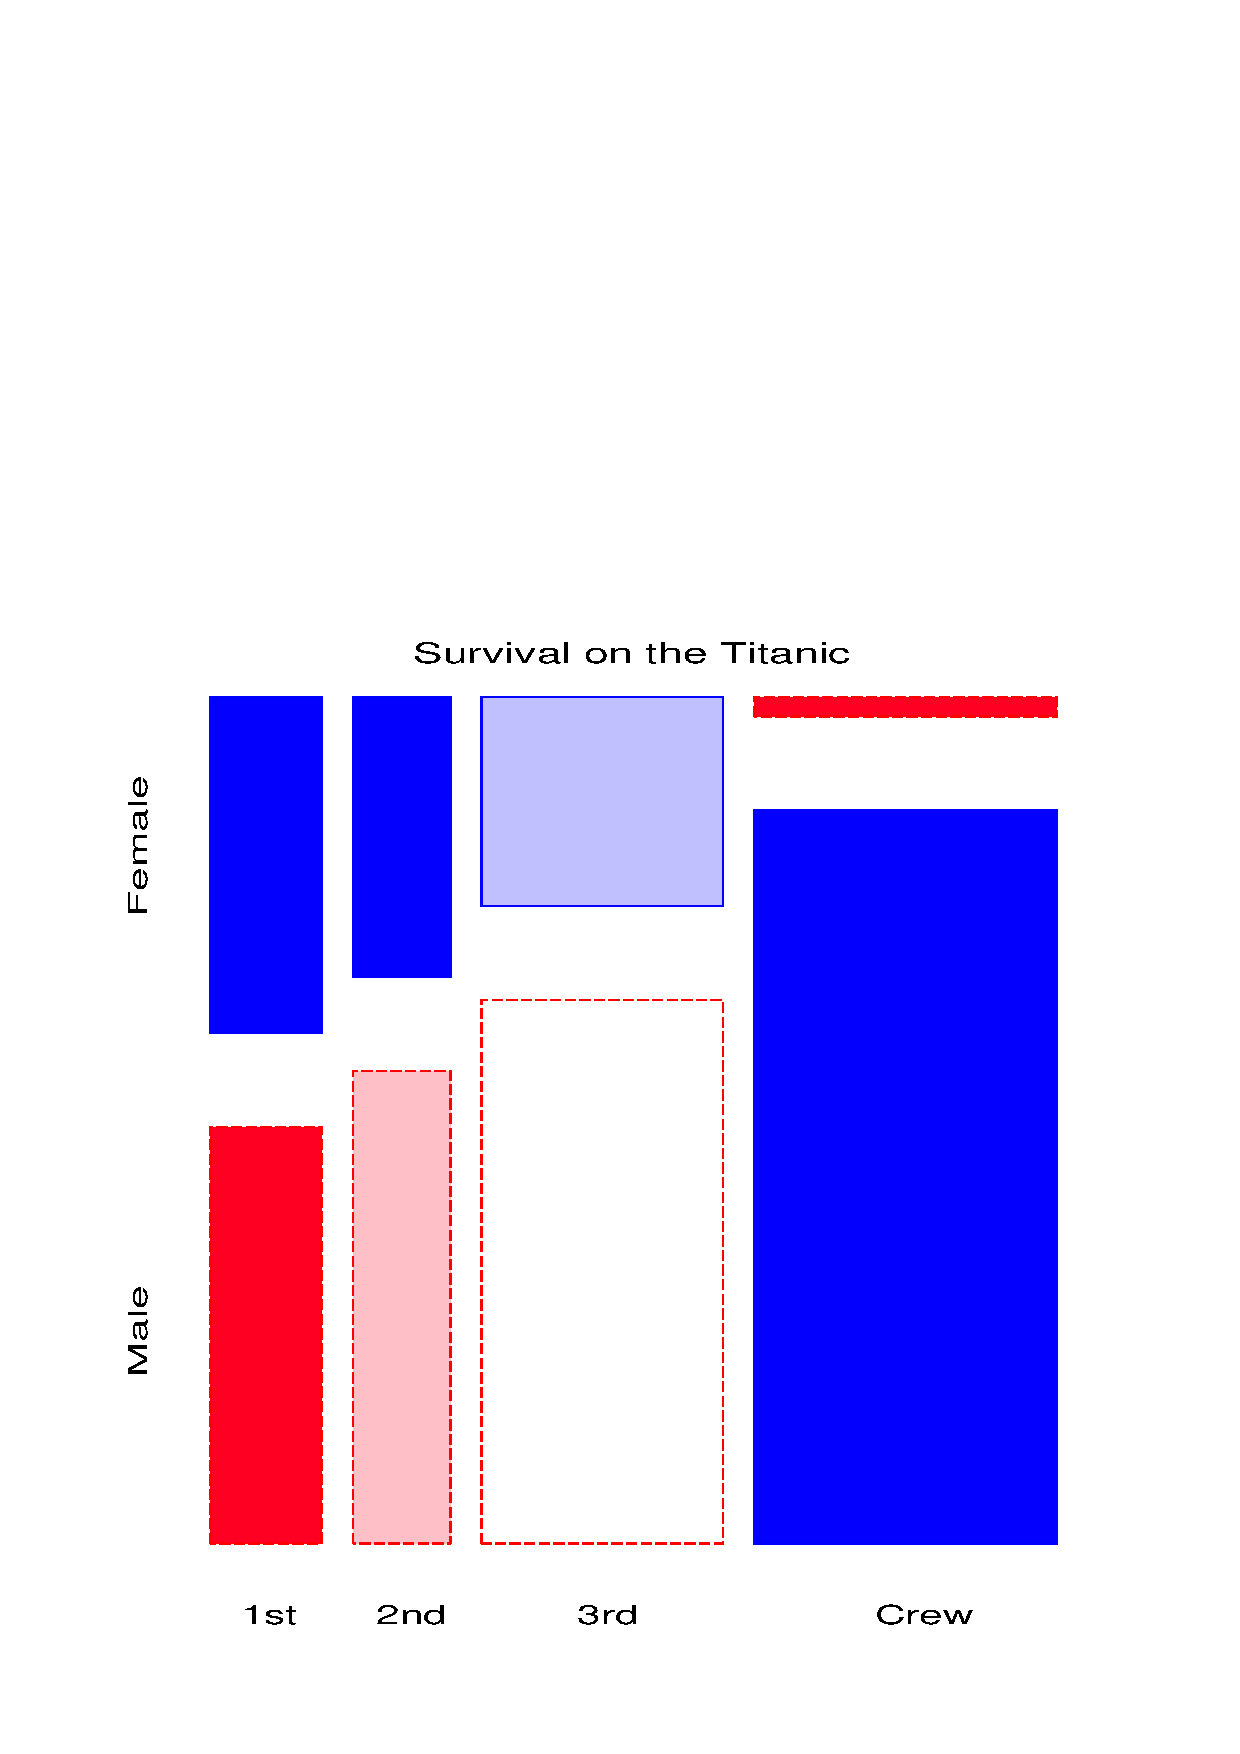
\includegraphics[width=1\linewidth,clip]{fig/mostitanic1}
 \end{minipage}%
 \hfill
 \begin{minipage}[c]{.44\dispwidth}
Class $\times$ Gender:
  \begin{itemize}
	\item \% males decreases with increasing economic class, 
	\item crew almost entirely male
  \end{itemize}
Sequential mosaics: understand associations among background variables
 \end{minipage}
\end{frame}

\begin{frame}
\frametitle{Survival on the \textit{Titanic}: Background variables}

 \begin{minipage}[c]{.55\dispwidth}
  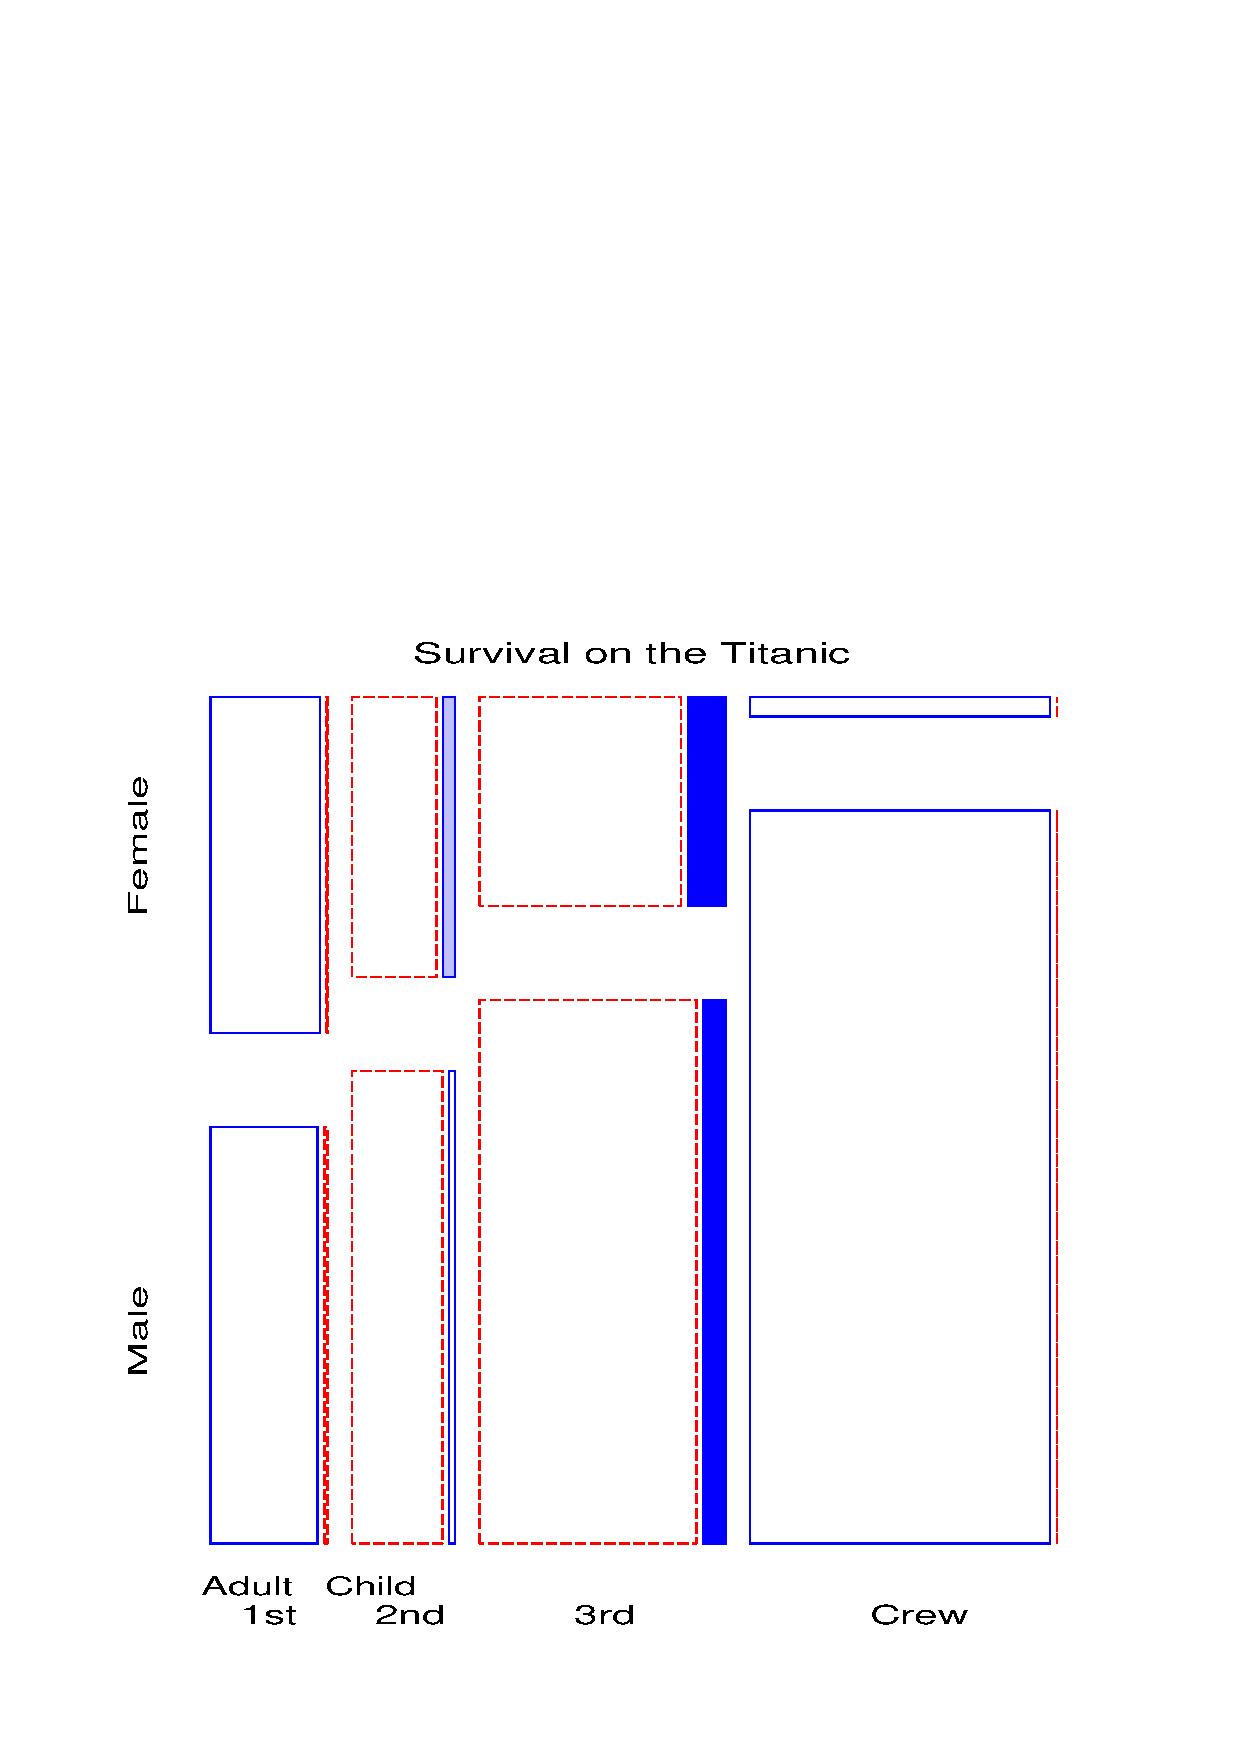
\includegraphics[width=1\linewidth,clip]{fig/mostitanic2}
 \end{minipage}%
 \hfill
 \begin{minipage}[c]{.44\dispwidth}
3 way: \{Class, Gender\} $\perp$ Age ?

  \begin{itemize}
	\item Overall proportion of children quite small (about 5 \%).
	\item \% children smallest in 1st class, largest in 3rd class.
	\item Residuals: greater number of children in 3rd class (families?)
  \end{itemize}
 \end{minipage}
\end{frame}

\begin{frame}
\frametitle{Survival on the \textit{Titanic}: 4 way table}

 \begin{minipage}[c]{.55\dispwidth}
  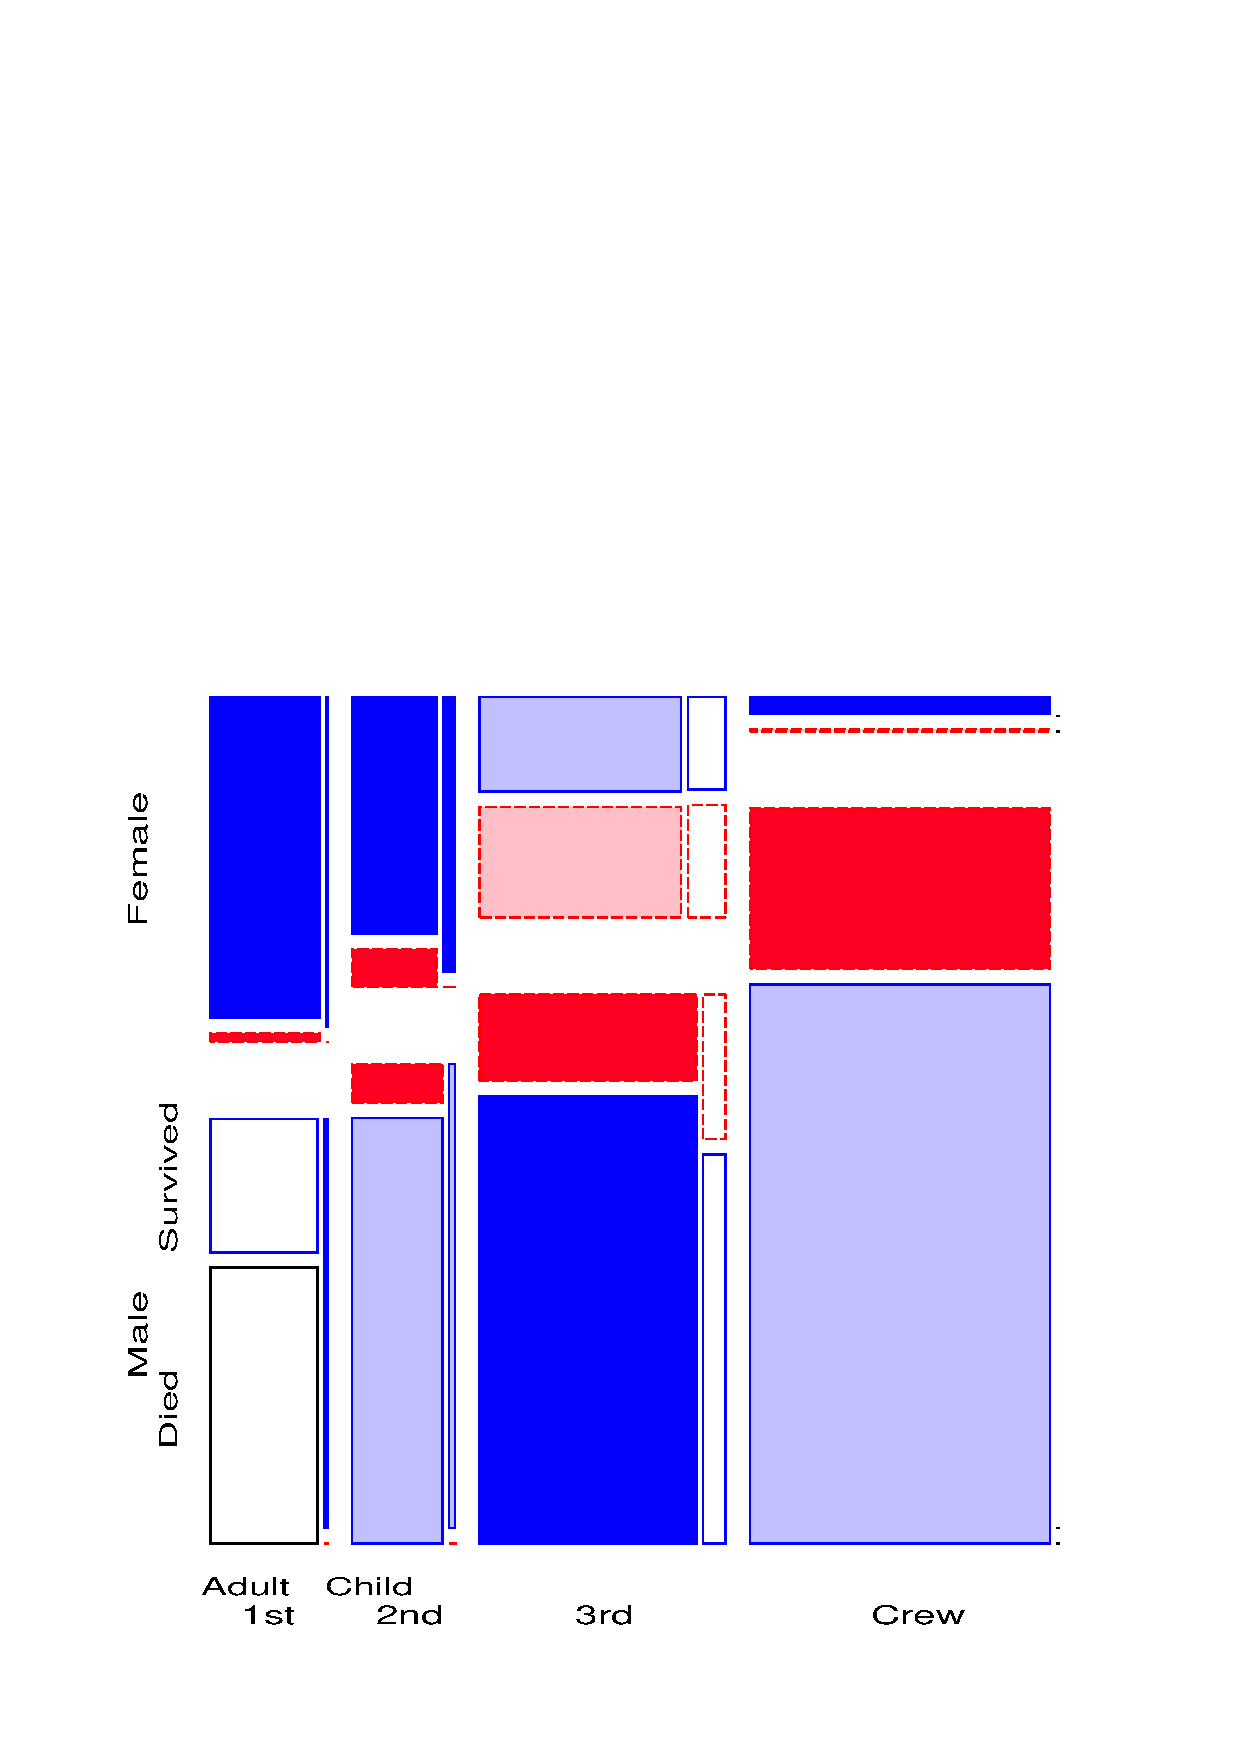
\includegraphics[width=1\linewidth,clip]{fig/mostitanic3}
 \end{minipage}%
 \hfill
 \begin{minipage}[c]{.44\dispwidth}
4 way:  \{Class, Gender, Age\} $\perp$ Survival ?

  \begin{itemize}
    \item Joint independence: [CGA][S]
	\item \alert{Minimal null model} when C, G, A are explanatory
	\item More women survived, but greater \% in 1st \& 2nd
	\item Among men,  \% survived increases with class.  
	\item Fits poorly [$G^2_{(15)} = 671.96$] $\Rightarrow$  \alert{Add $S$-assoc} terms
  \end{itemize}
 \end{minipage}
\end{frame}

\begin{frame}
\frametitle{Survival on the \textit{Titanic}: Better models}

 \begin{minipage}[c]{.5\dispwidth}
  \includegraphics[width=1\linewidth,clip]{fig/mostitanic5}
 \end{minipage}%
 \hfill
 \begin{minipage}[c]{.49\dispwidth}
	\textbf{women and children first} $\longrightarrow$
	\begin{itemize*}
    \item model $[CGA][\blue{\bm{CS}}][\blue{\bm{GAS}}]$ (Age and Gender affect survival, independent
	of Class)
	\item Model improved slightly, but still not good ($G^2_{(9)} = 94.54$).
	\end{itemize*}
 \end{minipage}
\end{frame}

\begin{frame}
\frametitle{Survival on the \textit{Titanic}: Better models}

 \begin{minipage}[c]{.5\dispwidth}
  \includegraphics[width=1\linewidth,clip]{fig/mostitanic6}
 \end{minipage}%
 \hfill
 \begin{minipage}[c]{.49\dispwidth}
	\textbf{Class interacts with Age \& Gender} on survival: 
	\begin{itemize*}
    \item Model $[CGA][\blue{\bm{CGS}}][\blue{\bm{CAS}}]$
	\item $G^2_{(4)}$ now 1.69, a very good fit.
    \item Perhaps too good? (Overfitting?) $\rightarrow$ check AIC!
	\end{itemize*}

 \end{minipage}
\end{frame}


\begin{frame}
\frametitle{\textit{Titanic} Conclusions}
Mosaic displays allow a detailed explanation:
\begin{itemize}
\item Regardless of Age and Gender, lower economic
status $\longrightarrow$  increased mortality.
\item Differences due to Class were moderated by both Age and Gender.
\item Women  more likely \emph{overall} to survive than men, but:
\begin{itemize*}
	\item  Class $\times$ Gender:
	women in 3rd class \emph{did not} have a significant advantage
	\item men in 1st class \emph{did}, compared to men in other classes.
\end{itemize*}

\item  Class $\times$ Age: 
\begin{itemize*}
	\item no children in 1st or 2nd class died, but
	\item nearly two-thirds of children in 3rd class died.
	\item For adults, mortality $\uparrow$ as economic class $\downarrow$.
\end{itemize*}

\item Summary statement:\newline
``\textbf{women and children (according to class), then 1st class men}''.
\end{itemize}
\end{frame}

\begin{frame}<beamer>
\frametitle{\textit{Titanic} Conclusions}
\begin{center}
New study, \emph{Proc. Nat. Acad. Sciences}, March, 2010:  
  \includegraphics[width=.78\textwidth]{fig/Titanic-Lusitania-head}\\
  \includegraphics[width=.78\textwidth]{fig/Titanic-Lusitania}
\end{center}
\end{frame}
\endinput

